\documentclass{scrartcl}
\usepackage[utf8]{inputenc}
\usepackage{tikz}
\usetikzlibrary{arrows,decorations.pathmorphing,backgrounds,fit,positioning,shapes.symbols,chains,shapes.geometric,shapes.arrows,calc}

\begin{document}
  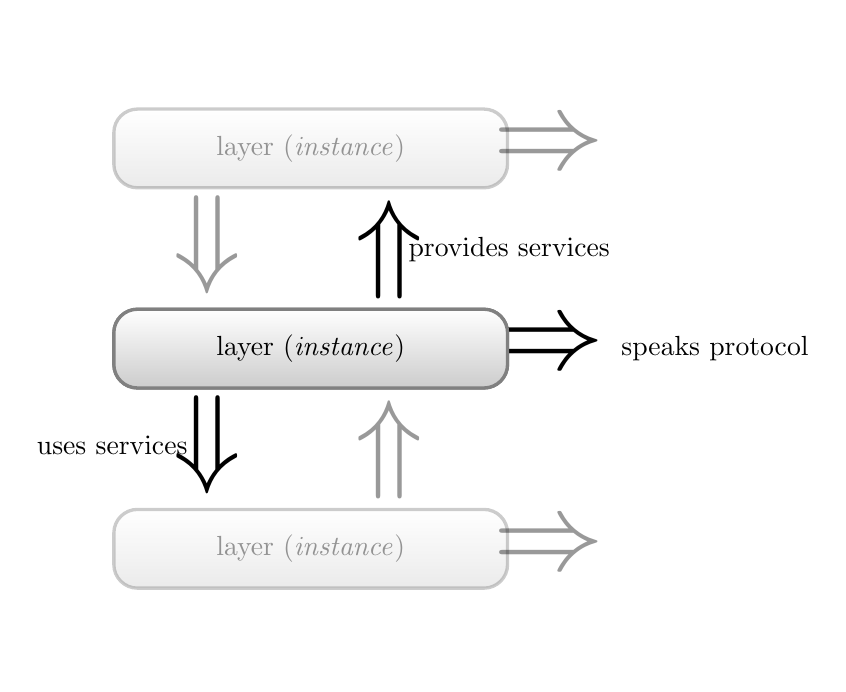
\begin{tikzpicture}
  [scale=0.5,
  schicht/.style={rectangle, minimum size=10mm,minimum width=50mm,rounded corners=3mm,very thick,draw=black!50,top color=white,bottom color=black!20},
  schicht2/.style={rectangle, minimum size=10mm,minimum width=50mm,rounded corners=3mm, very thick,draw=black!50, top color=white,bottom color=black!20, opacity=0.4}]
  \node (schicht)  [schicht] {layer (\textit{instance})};
  \node (Protokoll)  [right=1.3cm of schicht] {speaks protocol};
  \node (Dienste1) [above=0.98cm of schicht.east] {provides services};
  \node (Dienste2) [below=0.98cm of schicht.west] {uses services};
  \node [left=-0.8cm of Dienste1, scale=4] {$\Uparrow$};
  \node [right=-0.8cm of Dienste2, scale=4] {$\Downarrow$};
  \node [right=-0.7cm of schicht, scale=4] {$\Rightarrow$};
  \node (schicht1)  [schicht] {layer (\textit{instance})};
  \node (schicht2)  [schicht2, below=1.5cm of schicht] {layer (\textit{instance})};
  \node (Dienste3) [above=0.98cm of schicht2.east, opacity=0]{provides services};
  \node (Dienste4) [below=0.98cm of schicht2.west, opacity=0] {uses services};
  \node [left=-0.8cm of Dienste3, scale=4, opacity=0.4] {$\Uparrow$};
%  \node [right=-0.8cm of Dienste4, scale=4, opacity=0.4] {$\Downarrow$};
  \node [right=-0.7cm of schicht2, scale=4, opacity=0.4] {$\Rightarrow$};
  \node (schicht3)  [schicht2, above=1.5cm of schicht] {layer (\textit{instance})};
  \node (Dienste5) [above=0.98cm of schicht3.east, opacity=0]{provides services};
  \node (Dienste6) [below=0.98cm of schicht3.west, opacity=0] {uses services};
%  \node [left=-0.8cm of Dienste5, scale=4, opacity=0.4] {$\Uparrow$};
  \node [right=-0.8cm of Dienste6, scale=4, opacity=0.4] {$\Downarrow$};
  \node [right=-0.7cm of schicht3, scale=4, opacity=0.4] {$\Rightarrow$};
  \end{tikzpicture}
\end{document}
